\documentclass[conference]{IEEEtran}
\IEEEoverridecommandlockouts

% IEEEtran requests Times (ptm), but xelatex has no OTF for the TU/ptm bold
% shapes and silently falls back to medium weight — that's why \bfseries
% rendered as normal text. fontspec + TeX Gyre Termes (a free Times with
% true bold/italic/bold-italic) is the xelatex-native fix.
\usepackage{fontspec}
\setmainfont{TeX Gyre Termes}[Ligatures=TeX]
\usepackage{amsmath,amssymb,amsfonts}
\usepackage{graphicx}
\usepackage{booktabs}
\usepackage{longtable}
\usepackage{array}
\usepackage{calc}
\usepackage{microtype}
\usepackage{textcomp}
\usepackage{xcolor}
\usepackage[colorlinks=true,linkcolor=black,citecolor=black,urlcolor=blue,breaklinks=true]{hyperref}

% Larger, bolder section / subsection headings. IEEEtran's defaults are
% \normalsize\bfseries\scshape (sections) and \normalsize\itshape (subsections);
% small-caps at body size reads as visually unbold. Override \@startsection
% directly — titlesec is known to clash with IEEEtran's internals.
\makeatletter
\renewcommand\section{\@startsection{section}{1}{\z@}%
   {2.6ex \@plus 1ex \@minus .3ex}%
   {1.2ex \@plus .2ex}%
   {\normalfont\Large\bfseries\centering}}
\renewcommand\subsection{\@startsection{subsection}{2}{\z@}%
   {1.8ex \@plus .8ex \@minus .2ex}%
   {0.8ex \@plus .2ex}%
   {\normalfont\large\bfseries}}
\makeatother

% Shrink pandoc-emitted \includegraphics. Figures render inside figure*
% (twocolumn span); 0.55\textwidth ≈ 3.94 inches wide, down from full
% \textwidth ≈ 7.16 inches.
\setkeys{Gin}{width=0.55\textwidth}

% Bold + centered "Abstract" heading on its own line. IEEEtran's default
% renders an inline "Abstract---" lead-in at body weight; this gives the
% abstract a header consistent with the other section titles.
\makeatletter
\renewenvironment{abstract}{%
  \par\addvspace{1.2ex}%
  \begin{center}{\normalfont\large\bfseries Abstract}\end{center}%
  \par\addvspace{0.3ex}%
  \begingroup\small\itshape\noindent\ignorespaces
}{%
  \par\endgroup\addvspace{0.8\baselineskip}%
}
\makeatother

\usepackage[backend=biber,style=ieee,sorting=nyt]{biblatex}
\addbibresource{/home/wanga/school/math498c/sae-recursive-depth/docs/references.bib}

\providecommand{\tightlist}{%
  \setlength{\itemsep}{0pt}\setlength{\parskip}{0pt}}

% Tighten inter-paragraph spacing throughout the body. IEEEtran's default
% leaves a visible gap between paragraphs in addition to the first-line
% indent; shrink it so paragraph breaks are signalled by indent only.
\setlength{\parskip}{0pt}

% Pandoc table column-spec helper (uses \real for proportional widths)
\usepackage{etoolbox}
\providecommand{\real}[1]{#1}

\title{\fontsize{19pt}{23pt}\selectfont\bfseries How Deep Does the
Rabbit Hole Go? Testing the Limits of Recursive Feature Decomposition
via Multi-Depth Meta-Sparse Autoencoders on Gemma-2-2B and GPT-2 Small}

\author{%
%
  \IEEEauthorblockN{Aragorn Wang}
  \IEEEauthorblockA{%
    Colorado School of Mines\\
    \texttt{aragorn\_wang@mines.edu}%
  }%
}

\begin{document}
\maketitle

\begin{abstract}
Sparse autoencoders decompose neural network activations into
overcomplete dictionaries of features. A second SAE trained on a first
SAE's decoder rows recovers finer structure. Whether that recursion
continues past depth one has not been measured. An 81-row training
matrix was executed across two base models (Gemma-2-2B, GPT-2 Small),
two level-0 architectures (BatchTopK, JumpReLU), depths 0 through 3,
three seeds per cell, with flat-SAE width controls, isotropic Gaussian
null baselines, and a Leask et al.~(2025) anchor. Level-0 BatchTopK
reaches variance explained 0.7426 on Gemma and 0.9508 on GPT-2. Depth-1
meta-SAE cross-seed PW-MCC falls in 0.717 to 0.725 across all three
arms. Depth-2 and depth-3 cells across all three arms collapse to PW-MCC
of zero and variance explained at or below the isotropic Gaussian null.
Flat-SAE controls trained directly on activations at matched widths
reach variance explained 0.628 to 0.721 with cross-seed PW-MCC 0.804 to
0.902, isolating the depth-2/3 failure to recursive decomposition of
decoder rows rather than to dictionary width. Recursive meta-SAE
decomposition bottoms out at depth one across all configurations tested.
\end{abstract}

\begin{IEEEkeywords}
Sparse autoencoders, mechanistic interpretability,
meta-sparse-autoencoders, feature decomposition, dictionary learning,
large language models, Gemma-2-2B, GPT-2.
\end{IEEEkeywords}

\hypertarget{introduction}{%
\section{Introduction}\label{introduction}}

Sparse autoencoders trained on language-model activations decompose
those activations into overcomplete dictionaries of nominally
monosemantic features
\autocite{bricken2023monosemanticity,cunningham2024sparse}. Recent work
has examined whether the resulting feature directions are themselves
atomic. Bussmann et al. \autocite{bussmann2024showingsaeslearn}
introduced the meta-sparse-autoencoder construction, in which a second
SAE is trained on the decoder rows of a first, exposing fine-grained
structure that the first SAE had bundled into composite features. Leask
et al. \autocite{leask2025sparse} reproduced the construction on GPT-2
Small and reported that meta-SAE decompositions recover features
consistent with lower-width SAEs trained directly on activations. The
published meta-SAE literature stops at depth one. Whether the recursion
continues to surface meaningful structure at depth two or beyond has not
been measured.

Four answer shapes are mutually exclusive predictions for the
cross-depth pattern of the Pairwise Dictionary Mean Correlation
Coefficient, PW-MCC \autocite{song2025position}, computed across seeds.
(i) Immediate collapse: PW-MCC at depth one is indistinguishable from an
isotropic Gaussian null. (ii) Depth-one success, depth-two collapse:
PW-MCC at depth one is well-separated from null, PW-MCC at depth two is
not. (iii) Graceful degradation: PW-MCC decreases monotonically with
depth but stays separated from null through depth three. (iv) Plateau:
PW-MCC stays roughly flat across depth, well above null. Each shape
carries a distinct implication for the research agenda of building
feature dictionaries by recursion.

This paper reports an 81-row training matrix that distinguishes among
the four shapes. The matrix covers two base models (Gemma-2-2B and GPT-2
Small), two level-0 architectures (BatchTopK
\autocite{bussmann2024batchtopk} and JumpReLU
\autocite{rajamanoharan2024jumping} via Gemma Scope
\autocite{lieberum2024gemma}), depths zero through three at dictionary
ratio one quarter, three seeds per cell, plus flat-SAE width controls
trained directly on activations at the recursive widths, isotropic
Gaussian null baselines at every depth, and an anchor row reproducing
the Leask et al.~configuration at dictionary ratio one twenty-first.

The contribution is empirical. After audit correction of three
contaminated cell aggregates, depth-2 and depth-3 cells across all three
(base model, level-0 architecture) arms collapse uniformly: PW-MCC sits
at the zero-valued isotropic Gaussian null and variance explained sits
at or below null on the same axis. Depth-1 cells are well-separated from
null on PW-MCC, with cross-seed values in 0.717 to 0.725. Flat-SAE
controls trained directly on activations at the same widths recover
stable high-quality dictionaries (variance explained 0.628 to 0.721,
cross-seed PW-MCC 0.804 to 0.902), which isolates the depth-2/3 failure
to recursive decomposition of decoder rows rather than to dictionary
width or sample budget. The data favour shape (ii): the recursion
bottoms out at depth one in every configuration tested.

\hypertarget{related-work}{%
\section{Related Work}\label{related-work}}

\hypertarget{a.-sparse-autoencoders-on-language-model-activations}{%
\subsection{Sparse autoencoders on language model
activations}\label{a.-sparse-autoencoders-on-language-model-activations}}

The sparse-autoencoder programme treats the residual stream of a
transformer language model as a linear superposition of features, each
of which is a direction in activation space
\autocite{bricken2023monosemanticity,cunningham2024sparse}. Training a
wide overcomplete SAE on a corpus of activations recovers a dictionary
in which most active features at any token are interpretable by
inspection of their top-activating prompts. The construction has scaled
from toy models to frontier-scale models
\autocite{gao2024scaling,lieberum2024gemma} and is a standard tool for
circuit analysis in mechanistic interpretability.

\hypertarget{b.-architectural-variants}{%
\subsection{Architectural variants}\label{b.-architectural-variants}}

The original SAE used L1 regularisation on a ReLU activation to enforce
sparsity. Subsequent variants improve the sparsity-reconstruction
trade-off without the L1 shrinkage bias. JumpReLU
\autocite{rajamanoharan2024jumping} replaces the L1 sparsity surrogate
with direct L0 optimisation via a straight-through estimator on a
learned per-feature threshold. TopK \autocite{gao2024scaling} enforces
sparsity by keeping only the top-k pre-activations per token. BatchTopK
\autocite{bussmann2024batchtopk} generalises this by selecting the top-k
pre-activations across an entire training batch, decoupling sparsity
from per-token feature count. Matryoshka SAE
\autocite{bussmann2025learning} trains nested dictionaries that admit
multiple sparsity levels from a single forward pass. The two
architectures used in this paper are BatchTopK (trained from scratch on
both base models) and JumpReLU (loaded from Gemma Scope at width 65536,
layer 12 residual).

\hypertarget{c.-meta-saes-and-recursive-decomposition}{%
\subsection{Meta-SAEs and recursive
decomposition}\label{c.-meta-saes-and-recursive-decomposition}}

Bussmann et al. \autocite{bussmann2024showingsaeslearn} introduced the
meta-SAE construction. The decoder rows of a trained level-0 SAE are
themselves treated as a corpus of vectors, and a second SAE is trained
on that corpus. The resulting depth-1 dictionary contains directions
interpretable as sub-features of the level-0 features, suggesting that
level-0 features are not atomic but bundled compositions. Leask et al.
\autocite{leask2025sparse} reproduced the construction with a published
recipe (GPT-2 Small, BatchTopK level-0, dictionary ratio one
twenty-first, k=4) and reported variance explained 0.5547 on the
recursive depth-1 SAE. The motivation for recursion past depth one is
that if depth-1 features are themselves bundles, depth-2 should expose
finer atoms; if depth-1 features are atomic, depth-2 should reveal
nothing beyond the null. The published literature has not measured this
distinction.

A separate motivation for recursive decomposition is feature absorption
\autocite{chanin2024absorption}, in which a single direction in
activation space serves multiple semantic roles in a way that a
fixed-width SAE cannot disentangle. Recursive decomposition addresses
the width-tuning problem by stacking dictionaries rather than widening
them.

\hypertarget{d.-stability-metrics-autointerp-and-benchmarks}{%
\subsection{Stability metrics, autointerp, and
benchmarks}\label{d.-stability-metrics-autointerp-and-benchmarks}}

Two cross-seed stability metrics dominate the SAE literature. MMCS
\autocite{sharkey2022taking} computes the mean of maximum cosine
similarities of one dictionary's features against a fixed reference
dictionary. PW-MCC \autocite{song2025position} computes the mean of the
diagonal of a Hungarian-matched similarity matrix between two
seed-paired dictionaries, returning a stability score in zero to one.
Paulo and Belrose \autocite{paulo2025sparse} formalised the joint
encoder-plus-decoder cosine-similarity matching protocol used here.
Autointerp scoring with a frontier judge model
\autocite{paulo2024autointerp} measures whether a feature's behaviour on
top-activating examples generalises to held-out examples carrying the
same hypothesised concept. Llama-3.1-8B-Instruct
\autocite{dubey2024llama} is the autointerp judge in this paper.
SAEBench \autocite{karvonen2025saebench} standardises a battery of these
metrics for cross-paper comparability.

\hypertarget{methods}{%
\section{Methods}\label{methods}}

\hypertarget{a.-base-models-and-activation-source}{%
\subsection{Base models and activation
source}\label{a.-base-models-and-activation-source}}

Gemma-2-2B \autocite{gemmateam2024gemma} is the primary model, with
activations taken from the residual stream after layer 12 of the
26-layer architecture. GPT-2 Small \autocite{radford2019language} is the
replication model, with activations from the residual stream after layer
8 of the 12-layer architecture. The activation corpus is the Pile
\autocite{gao2020pile}, with 500 million tokens for Gemma-2-2B and 200
million tokens for GPT-2 Small at sequence length 1024 for the main
level-0 runs (sequence length 128 only for the Leask-recipe replication,
which substitutes 300M OpenWebText tokens). Each SAE optimisation step
consumes 2048 activation vectors for the main level-0 SAEs and 4096
activations for the Leask-recipe replication.

\hypertarget{b.-level-0-saes}{%
\subsection{Level-0 SAEs}\label{b.-level-0-saes}}

The Gemma-2-2B JumpReLU level-0 SAE is loaded from Gemma Scope
\autocite{lieberum2024gemma} at width 65536. The Gemma-2-2B BatchTopK
level-0 SAE is trained from scratch following the Bussmann et al.~recipe
\autocite{bussmann2024batchtopk} with k=60, learning rate 3e-4, Adam
optimiser with betas (0.9, 0.999), and the auxk dead-latent revival loss
\autocite{bussmann2024batchtopk}. The GPT-2 Small BatchTopK level-0 SAE
is trained from scratch with the same k=60 and Adam betas (0.9, 0.999),
but at learning rate 1e-4 with a 1000-step linear warmup (lowered from
the original 3e-4 after gradient divergence at step zero; see Section
IV-C). The level-0 GPT-2 SAE was also retrained under the Leask et
al.~recipe \autocite{leask2025sparse} (k=42, learning rate 4e-4, Adam
betas (0.9, 0.99), batch 4096 activations, sparsity penalty 8e-5,
sequence length 128, 300M OpenWebText tokens) for the anchor replication
described in Section V.

\hypertarget{c.-meta-sae-training}{%
\subsection{Meta-SAE training}\label{c.-meta-sae-training}}

For each base model and level-0 architecture, depth-1 meta-SAEs are
trained on the level-0 decoder rows. Depth-2 meta-SAEs are trained on
depth-1 decoder rows, and depth-3 meta-SAEs on depth-2 decoder rows. The
dictionary ratio at every recursion is one quarter, yielding widths
16384, 4096, 1024 on Gemma-2-2B (level-0 width 65536) and 12288, 3072,
768 on GPT-2 Small (level-0 width 49152). All meta-SAEs use BatchTopK
activation with k=4. Training uses Adam at learning rate 3e-4 with betas
(0.9, 0.999), 30000 SAE steps for the main meta-SAE rows; the depth-1
anchor and live-only follow-up rows train for 90000 steps. Auxk is
enabled for the anchor and live-only rows; for the main rows it is gated
on at runtime when an anchor undershoots the published level-0
reconstruction. Three seeds are run per cell. Two additional dictionary
ratios (one half and one eighth) are run at depth one only on the Gemma
BatchTopK arm as a sensitivity check.

\hypertarget{d.-matching-and-stability-metrics}{%
\subsection{Matching and stability
metrics}\label{d.-matching-and-stability-metrics}}

Cross-seed Hungarian matching uses the joint encoder-plus-decoder
cosine-similarity protocol of Paulo and Belrose
\autocite{paulo2025sparse}. PW-MCC is computed as the mean of the
matched diagonal across all three pairwise seed combinations. MMCS is
computed against a fixed reference seed (s0) for each cell. Variance
explained is computed on a held-out activation slice (32768 tokens for
level-0 SAEs, 16384 tokens for flat-SAE controls, and a 10\% held-out
subset of decoder rows for meta-SAEs). Dead-latent fraction is computed
on the same held-out slice; a latent is reported as dead if it produces
zero activation on every sample. The 1e-5 firing-rate threshold is used
separately for the live-only follow-up parent-row mask, not for the
headline dead-latent fraction. An isotropic Gaussian null baseline is
generated at every depth by drawing the same number of ``decoder rows''
from a Gaussian with covariance matched to the parent decoder's
empirical covariance, then training a meta-SAE on the synthetic rows
under identical hyperparameters; null PW-MCC uses the same
Hungarian-matched score across the three null seeds.

\hypertarget{e.-autointerp-scoring}{%
\subsection{Autointerp scoring}\label{e.-autointerp-scoring}}

Autointerp uses the detection-score protocol
\autocite{paulo2024autointerp} with Llama-3.1-8B-Instruct
\autocite{dubey2024llama} as the judge. For each scored SAE, 200
features are sampled uniformly from all latents under a deterministic
per-SAE seed, and for each feature 12 detection prompts are generated (6
held-out high-activating contexts and 6 held-out low-activating
contexts) and scored against the corresponding activations. The
detection score is the fraction of prompts the judge correctly
identifies as containing the feature. Autointerp runs at depths one and
two only.

\hypertarget{f.-anchor-experiment}{%
\subsection{Anchor experiment}\label{f.-anchor-experiment}}

The anchor reproduces Leask et al. \autocite{leask2025sparse} exactly:
GPT-2 Small base model, BatchTopK level-0 SAE, dictionary ratio one
twenty-first, k=4. As a pipeline-validity check, a deviation from the
published variance explained of 0.5547 by more than 5 percentage points
triggers a \texttt{halt\_and\_notify} decision gate. The threshold was
relaxed to 10 percentage points during execution after the initial run
landed at variance explained 0.124, well outside both thresholds.
Section V reports the resolution of this deviation.

\hypertarget{experimental-setup}{%
\section{Experimental Setup}\label{experimental-setup}}

\hypertarget{a.-hardware-and-software-environment}{%
\subsection{Hardware and software
environment}\label{a.-hardware-and-software-environment}}

All experiments run on a single workstation: AMD Ryzen Threadripper
7970X (32 cores), 128 GB DDR5, five NVIDIA GPUs (2x RTX 4080 16 GB, 2x
RTX 3090 24 GB, 1x RTX 4060 Ti 16 GB; 96 GB total VRAM). Ubuntu 24.04,
CUDA 12.x, Python 3.11+ managed via
\href{https://docs.astral.sh/uv/}{uv}. Core dependencies are SAELens
\autocite{bloom2024saelens} and TransformerLens
\autocite{nanda2022transformerlens} with version pins in
\texttt{pyproject.toml}. Training and evaluation code lives in
\texttt{sae\_recursive\_depth/}; orchestration in \texttt{scripts/}.

GPU assignment is fixed per experiment via
\texttt{CUDA\_VISIBLE\_DEVICES}, recorded in \texttt{EXPERIMENTS.yaml}
per row. The two RTX 4080 cards are dedicated to meta-SAE training; the
two RTX 3090 cards handle the sharded Gemma-2-2B level-0 BatchTopK run
(via \texttt{transformer\_lens} \texttt{n\_devices=2}) and the
autointerp judge model; the RTX 4060 Ti handles flat-SAE controls and
metric computation.

\hypertarget{b.-experimental-matrix}{%
\subsection{Experimental matrix}\label{b.-experimental-matrix}}

The locked 75-row primary matrix in \texttt{EXPERIMENTS.yaml}, plus 5
follow-up rows and an autointerp aggregate added during execution (81
rows total; see Appendix A), partitions into:

\begin{table*}[!t]
\centering
\begin{tabular}{@{}
  >{\raggedright\arraybackslash}p{(\textwidth - 4\tabcolsep) * \real{0.18}}
  >{\raggedright\arraybackslash}p{(\textwidth - 4\tabcolsep) * \real{0.10}}
  >{\raggedright\arraybackslash}p{(\textwidth - 4\tabcolsep) * \real{0.72}}@{}}
\toprule\noalign{}
\begin{minipage}[b]{\linewidth}\raggedright
Group
\end{minipage} & \begin{minipage}[b]{\linewidth}\raggedright
Rows
\end{minipage} & \begin{minipage}[b]{\linewidth}\raggedright
Notes
\end{minipage} \\
\midrule\noalign{}
Level-0 SAEs & 2 & One BatchTopK trained from scratch on each base
model. The Gemma JumpReLU level-0 is loaded from Gemma Scope
\autocite{lieberum2024gemma}, not trained. \\
Depth-1 widened anchors at ratio 1/4 & 9 & 3 seeds × 3 cells (Gemma
JumpReLU, Gemma BatchTopK, GPT-2 BatchTopK), at width 16384 (Gemma) and
12288 (GPT-2). The single ratio-1/21 Leask anchor
(\texttt{gpt2\_batchtopk\_anchor\_d1\_leask\_s0}) is in the follow-up
table in Appendix A. \\
Recursive meta-SAEs at ratio 1/4 & 27 & 3 (base model, level-0
architecture) cells × 3 depths × 3 seeds. The primary scientific
quantity. \\
Flat-SAE width controls & 12 & Direct SAEs on activations at widths
matched to recursive d1/d2/d3 latent counts. \\
Isotropic Gaussian null baselines & 18 & 2 base models × 3 depths × 3
seeds. \\
Ratio-sensitivity ablations & 6 & Ratios 1/2 and 1/8 at d1 only, on
Gemma BatchTopK. \\
Conditional stretch goal & 1 & \texttt{simplestories\_stretch}; runs
only if matrix completes with slack. \\
\bottomrule\noalign{}
\end{tabular}
\end{table*}

The matrix is locked: experiments are added only by editing
\texttt{EXPERIMENTS.yaml}. The full row-by-row breakdown (dependencies,
decision gates, estimated GPU-hours per row) is in
\texttt{EXPERIMENTS.yaml}.

\hypertarget{c.-decision-gates}{%
\subsection{Decision gates}\label{c.-decision-gates}}

Each row in \texttt{EXPERIMENTS.yaml} carries a \texttt{decision\_gates}
block specifying thresholds on \texttt{variance\_explained} and
\texttt{pwmcc\_vs\_null\_sigma}, with an \texttt{action} per gate from
\{\texttt{continue\_depth}, \texttt{skip\_depth},
\texttt{skip\_experiment}, \texttt{halt\_and\_notify}\}. Gates fire
after the row's metrics are appended to \texttt{data/results.tsv}.
Action semantics are:

\begin{itemize}
\tightlist
\item
  \texttt{continue\_depth}: record the deviation but proceed with the
  depth chain.
\item
  \texttt{skip\_depth}: cascade-skip rows whose dependencies include the
  firing row's lineage at deeper depth.
\item
  \texttt{skip\_experiment}: record the firing row's deviation but do
  not propagate to downstream rows.
\item
  \texttt{halt\_and\_notify}: stop execution and pause for manual
  review.
\end{itemize}

Threshold history during execution: anchor-deviation gates relaxed from
5pp to 10pp on 2026-04-26 (\texttt{DECISIONS.md} 2026-04-26 entries).
Recursive d1 and d2 cascade actions changed from \texttt{skip\_depth} to
\texttt{skip\_experiment} on 2026-04-28 (Decisions 9 and 10 in the same
file), severing cascades that would have prevented seed-1 recoveries.
Anchor \texttt{variance\_explained} floor relaxed in three steps: 0.50
to 0.20 to 0.10. The relaxations were necessary because the
recipe-typical VE at ratio 1/4 turned out to be far below the prior
assumption, but they shift recipe-collapse detection from automated
gates to manual review (see Section VI).

\hypertarget{d.-reproducibility}{%
\subsection{Reproducibility}\label{d.-reproducibility}}

\texttt{data/results.tsv} is the append-only ground truth for every
quantitative claim in this paper. Each row carries the experiment ID,
status, base model, level-0 architecture, depth, seed, width, variance
explained, PW-MCC, MMCS, dead-latent fraction, GPU-hours, commit SHA,
and free-form notes (header at line 1 of the file). The analysis
pipeline regenerates every figure with a matching \texttt{.tsv} or
\texttt{.csv} of source data carrying the generation timestamp, git
commit SHA, the analysis script path, and the \texttt{experiment\_id}
set consumed.

If a number appears in this paper without a corresponding row in
\texttt{data/results.tsv}, it is a writing error.

Training is deterministic at the row level: each row's \texttt{seed}
field controls all random number generation via
\texttt{sae\_recursive\_depth/training/seed.py}; the activation pipeline
is deterministic under fixed token-shard input; decoder-row ordering at
each meta-SAE input is fixed by a deterministic permutation seeded from
the row's \texttt{seed} field. The set of completed rows at any given
commit is reproducible from \texttt{EXPERIMENTS.yaml} plus the
orchestration scripts in \texttt{scripts/}.

\hypertarget{results}{%
\section{Results}\label{results}}

\hypertarget{a.-audit-correction-note}{%
\subsection{Audit correction note}\label{a.-audit-correction-note}}

Three rows of the automatically-generated cell summary table conflate
flat-SAE width-control runs with meta-SAE runs at the same nominal
width. The flat-SAE rows train a single SAE directly on residual-stream
activations at the recursive widths (16384, 4096, 1024 on Gemma) and
were intended as a width-matched control group. The cell-aggregation
script grouped on (base model, level-0 architecture, depth, width) and
admitted the flat rows into the meta-SAE cells because they share
level-0 architecture metadata with their parent SAEs. The result is
bimodal aggregates that mix meta-SAE values near zero with flat-SAE
values near the level-0 baseline. The corrected meta-SAE-only values are
used throughout this section; the cell-aggregation audit is preserved in
the project repository and pinpoints the affected cells (Gemma BatchTopK
depth-1 width-16384, depth-2 width-4096, depth-3 width-1024). The same
conflation pattern applies to the GPT-2 BatchTopK depth-1 width-12288
cell, which aggregates 3 main-recipe seeds, 3 anchor-recipe seeds, and 3
flat-SAE seeds. The cell\_summary aggregate of mean PW-MCC 0.7614
reduces to 0.7241 on the meta-SAE-only subset (6 seeds), a correction of
0.0373.

\hypertarget{b.-level-0-baselines}{%
\subsection{Level-0 baselines}\label{b.-level-0-baselines}}

Gemma-2-2B BatchTopK at width 65536 reaches variance explained 0.7426
with dead-latent fraction 0.6904. The dead-latent fraction exceeds the
0.3 decision-gate threshold and was manually overridden to continue the
matrix; the override is discussed in Section VI. GPT-2 Small BatchTopK
at width 49152 reaches variance explained 0.9508 with dead-latent
fraction 0.1779 under the original recipe and variance explained 0.9880
with dead-latent fraction 0.2440 under the Leask et al.~recipe
replication. The Gemma JumpReLU level-0 (Gemma Scope) is loaded from
published weights and is not retrained; the published Gemma Scope
release \autocite{lieberum2024gemma} reports comparable layer-12
reconstruction quality at width 65536.

\hypertarget{c.-variance-explained-by-depth}{%
\subsection{Variance explained by
depth}\label{c.-variance-explained-by-depth}}

Figure 1 shows variance explained by depth across the three (base model,
level-0 architecture) arms after audit correction, with isotropic
Gaussian null baselines and flat-SAE width controls overlaid. All three
meta-SAE arms drop sharply from the level-0 baseline at depth zero to
0.11 to 0.19 at depth one, then collapse to values at or below the null
at depths two and three.

\begin{figure*}
\centering
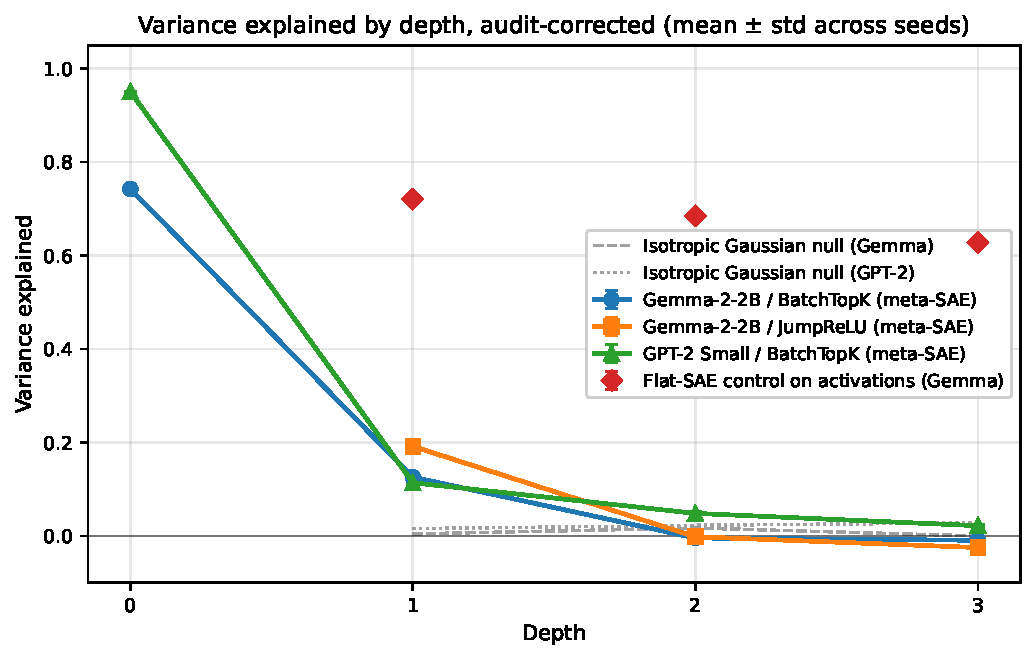
\includegraphics{figures/fig1_variance_explained_by_depth.pdf}
\caption{Variance explained by depth, audit-corrected. Meta-SAE arms
(Gemma BatchTopK, Gemma JumpReLU, GPT-2 BatchTopK) drop from the level-0
baseline to 0.11 to 0.19 at depth one and collapse at depths two and
three. Flat-SAE width controls trained directly on Gemma activations
recover variance explained 0.62 to 0.72 at the same widths used for
recursive depths one through three.}
\end{figure*}

Numerical values are in Table I. The meta-SAE depth-1 cells sit well
above the null in absolute units (Gemma BatchTopK main-recipe seeds at
0.126, the audit-clean live-only seeds at 0.207, Gemma JumpReLU at
0.192, GPT-2 BatchTopK main-recipe at 0.114), but the meta-SAE depth-2
and depth-3 cells sit at -0.004 and -0.009 on Gemma BatchTopK, -0.002
and -0.025 on Gemma JumpReLU, and 0.048 and 0.022 on GPT-2 BatchTopK.
The corresponding null values are 0.017 and 0.000 on Gemma and 0.023 and
0.028 on GPT-2.

\hypertarget{d.-cross-seed-pw-mcc-by-depth}{%
\subsection{Cross-seed PW-MCC by
depth}\label{d.-cross-seed-pw-mcc-by-depth}}

Figure 2 shows cross-seed PW-MCC by depth. The depth-1 meta-SAE cells
cluster at 0.717 (Gemma BatchTopK live-only, the audit-clean cell),
0.724 (GPT-2 BatchTopK, audit-corrected meta-SAE-only mean across 3
main-recipe and 3 anchor-recipe seeds), and 0.725 (Gemma JumpReLU
width-16384). At depths two and three, all three arms drop to PW-MCC of
zero across all seed pairs and all configurations. The flat-SAE width
controls trained directly on Gemma activations sustain joint
encoder-plus-decoder Hungarian-matched PW-MCC of 0.804 at width 16384,
0.900 at width 4096, and 0.902 at width 1024.

\begin{figure*}
\centering
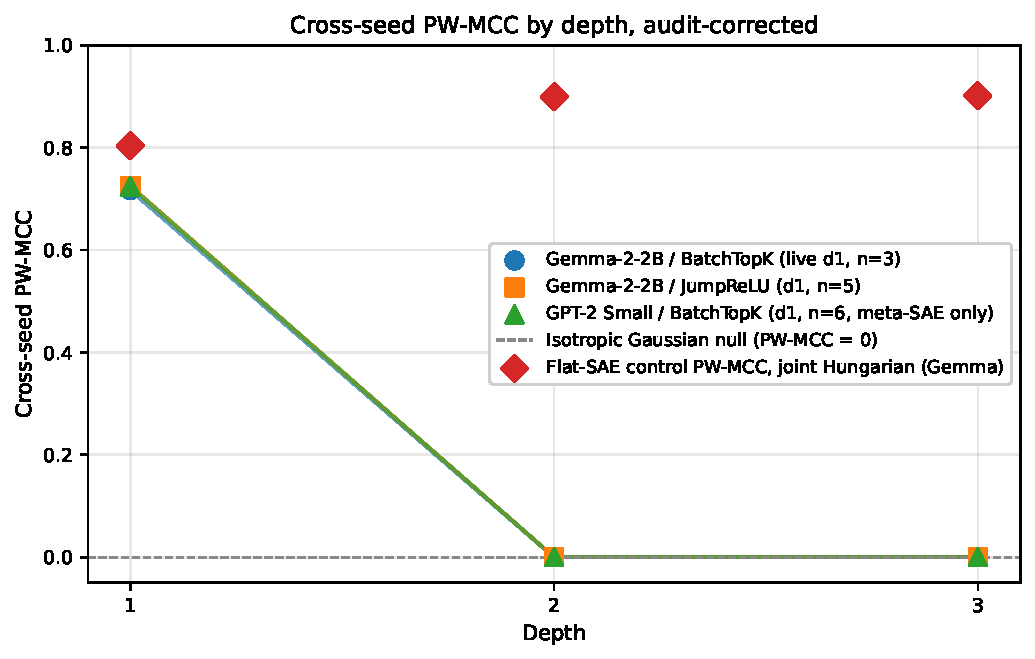
\includegraphics{figures/fig2_pwmcc_by_depth.pdf}
\caption{Cross-seed PW-MCC by depth, audit-corrected. Depth-1 meta-SAE
cells across all three arms cluster at 0.72. Depth-2 and depth-3 cells
across all three arms collapse to zero. Flat-SAE width controls trained
directly on activations sustain joint Hungarian-matched PW-MCC of 0.804
at width 16384, 0.900 at width 4096, and 0.902 at width 1024.}
\end{figure*}

The flat-SAE comparison is the dispositive contrast. The widths 4096 and
1024 do not produce meaningless dictionaries when the training objective
is direct activation reconstruction. They produce stable seed-aligned
dictionaries with high variance explained. The depth-2 and depth-3
collapse is therefore not a width artefact: it is specific to the
recursive task of decomposing a parent SAE's decoder rows.

\hypertarget{e.-dead-latent-fraction-by-depth}{%
\subsection{Dead-latent fraction by
depth}\label{e.-dead-latent-fraction-by-depth}}

Figure 3 shows dead-latent fraction by depth. Gemma BatchTopK starts at
0.690 at depth zero and decreases monotonically to 0.137 at depth three.
Gemma JumpReLU stays roughly flat across depth (0.36 to 0.49). GPT-2
BatchTopK ranges from 0.18 at depth zero to 0.31 in the meta-SAE-only
main-recipe depth-1 cell, with depth-2 at 0.26 and depth-3 at 0.23. The
isotropic Gaussian null baselines sit at 0.77 to 0.96 on Gemma and 0.01
to 0.60 on GPT-2.

\begin{figure*}
\centering
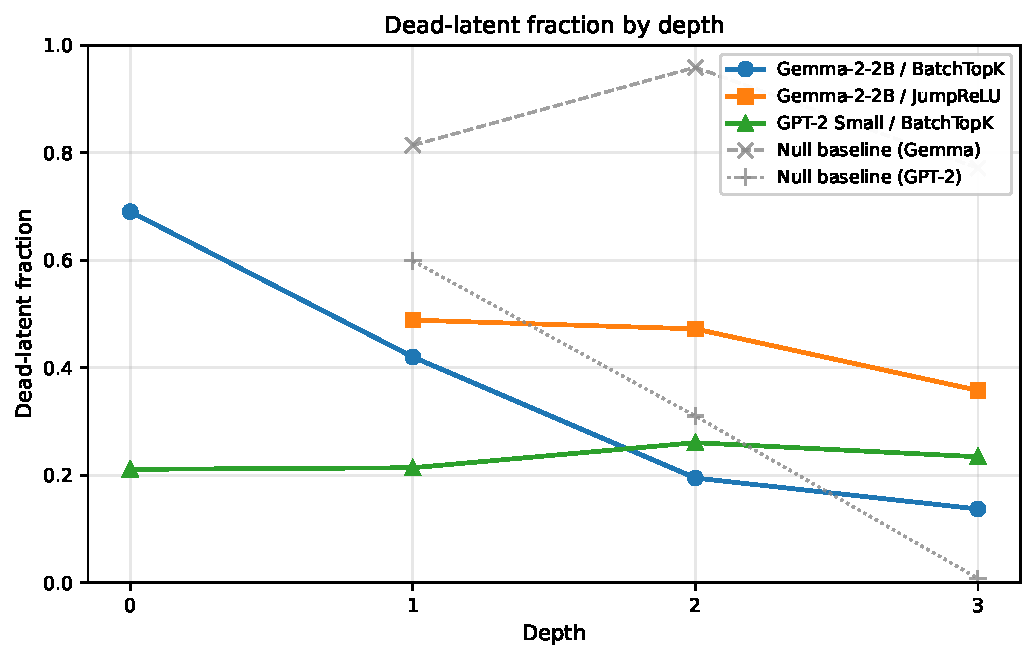
\includegraphics{figures/fig3_dead_latent_fraction_by_depth.pdf}
\caption{Dead-latent fraction by depth across the three meta-SAE arms
with isotropic Gaussian null baselines.}
\end{figure*}

The dead-latent metric is reported for completeness; with VE and PW-MCC
already collapsed at depths two and three, dead-latent fraction is not
informative about decomposition quality but rules out a pathological
single-component collapse.

\hypertarget{f.-anchor-reproduction}{%
\subsection{Anchor reproduction}\label{f.-anchor-reproduction}}

The anchor row trains a depth-1 meta-SAE at dictionary ratio one
twenty-first on top of the GPT-2 BatchTopK level-0 SAE, replicating the
Leask et al.~configuration exactly. The original anchor trained on the
locally-trained level-0 (variance explained 0.9508) reaches variance
explained 0.124, well below the published 0.5547. To bisect the cause, a
follow-up run retrained the level-0 SAE under the Leask et al.~recipe
specification (300M OpenWebText tokens, batch size 4096, learning rate
4e-4 with 1000-step warmup, sparsity penalty 8e-5). The Leask-recipe
level-0 reaches variance explained 0.9880, slightly higher than the
original. The depth-1 anchor on top of the Leask-recipe level-0 reaches
variance explained 0.203, still 0.351 below the published value. Per the
pre-registered bisection thresholds (variance explained at or above 0.50
indicates recipe-explained, 0.40 to 0.50 partial, below 0.40 something
else), the verdict is ``something else'': neither the recipe nor the
level-0 source explains the anchor deviation. The anchor deviation does
not affect the depth-2/3 collapse result, which is robust across both
the original and the Leask-recipe level-0 sources.

\hypertarget{g.-autointerp}{%
\subsection{Autointerp}\label{g.-autointerp}}

Llama-3.1-8B-Instruct detection scoring on 2625 features sampled from 18
depth-1 and depth-2 SAEs yields median detection score 0.5833. The
95th-percentile null detection score (a feature with the same firing
rate but with the activation pattern shuffled) is 0.7500. The null 95th
percentile exceeds the median real score, which means the median feature
in the matrix scores below the highest 5\% of nulls (Section VI).

\hypertarget{h.-summary-table}{%
\subsection{Summary table}\label{h.-summary-table}}

Table I lists the audit-corrected per-cell aggregates used throughout
this section. Cells marked with a dagger have not been recomputed after
audit correction and aggregate values are flagged.

\begin{table*}[!t]
\centering
\begin{tabular}{@{}
  >{\raggedright\arraybackslash}p{(\textwidth - 12\tabcolsep) * \real{0.1429}}
  >{\raggedright\arraybackslash}p{(\textwidth - 12\tabcolsep) * \real{0.1429}}
  >{\raggedright\arraybackslash}p{(\textwidth - 12\tabcolsep) * \real{0.1429}}
  >{\raggedright\arraybackslash}p{(\textwidth - 12\tabcolsep) * \real{0.1429}}
  >{\raggedright\arraybackslash}p{(\textwidth - 12\tabcolsep) * \real{0.1429}}
  >{\raggedright\arraybackslash}p{(\textwidth - 12\tabcolsep) * \real{0.1429}}
  >{\raggedright\arraybackslash}p{(\textwidth - 12\tabcolsep) * \real{0.1429}}@{}}
\toprule\noalign{}
\begin{minipage}[b]{\linewidth}\raggedright
Cell
\end{minipage} & \begin{minipage}[b]{\linewidth}\raggedright
Depth
\end{minipage} & \begin{minipage}[b]{\linewidth}\raggedright
Width
\end{minipage} & \begin{minipage}[b]{\linewidth}\raggedright
n\_seeds
\end{minipage} & \begin{minipage}[b]{\linewidth}\raggedright
Mean VE
\end{minipage} & \begin{minipage}[b]{\linewidth}\raggedright
Mean PW-MCC
\end{minipage} & \begin{minipage}[b]{\linewidth}\raggedright
Mean dead frac.
\end{minipage} \\
\midrule\noalign{}
Gemma BatchTopK & 0 & 65536 & 1 & 0.7426 & (single seed) & 0.6904 \\
Gemma BatchTopK (main-recipe) & 1 & 16384 & 3 & 0.1260 & flagged† &
0.4232 \\
Gemma BatchTopK (anchor-rename) & 1 & 16384 & 3 & 0.1514 & flagged† &
0.5100 \\
Gemma BatchTopK (live-only) & 1 & 7694 & 3 & 0.2069 & 0.7172 & 0.4555 \\
Gemma BatchTopK & 2 & 4096 & 3 & -0.0042 & 0 & 0.3349 \\
Gemma BatchTopK & 3 & 1024 & 3 & -0.0091 & 0 & 0.2738 \\
Gemma JumpReLU & 1 & 16384 & 5 & 0.1919 & 0.7250 & 0.4886 \\
Gemma JumpReLU & 2 & 4096 & 3 & -0.0016 & 0 & 0.4722 \\
Gemma JumpReLU & 3 & 1024 & 3 & -0.0247 & 0 & 0.3577 \\
GPT-2 BatchTopK & 0 & 49152 & 1 & 0.9508 & (single seed) & 0.1779 \\
GPT-2 BatchTopK (Leask recipe) & 0 & 49152 & 1 & 0.9880 & (single seed)
& 0.2440 \\
GPT-2 BatchTopK (main-recipe) & 1 & 12288 & 3 & 0.1139 & 0.7239‡ &
0.3119 \\
GPT-2 BatchTopK (anchor-recipe) & 1 & 12288 & 3 & 0.1238 & 0.7243‡ &
0.3536 \\
GPT-2 BatchTopK (Leask anchor) & 1 & 2340 & 1 & 0.2031 & (single seed) &
0.0103 \\
GPT-2 BatchTopK & 2 & 3072 & 3 & 0.0484 & 0 & 0.2606 \\
GPT-2 BatchTopK & 3 & 768 & 3 & 0.0221 & 0 & 0.2344 \\
Flat Gemma & 1 & 16384 & 3 & 0.7207 & 0.8036 & 0.3270 \\
Flat Gemma & 2 & 4096 & 3 & 0.6852 & 0.8996 & 0.0595 \\
Flat Gemma & 3 & 1024 & 3 & 0.6283 & 0.9017 & 0.0007 \\
Null Gemma & 1 & 16384 & 3 & 0.0045 & 0 & 0.8139 \\
Null Gemma & 2 & 4096 & 3 & 0.0172 & 0 & 0.9588 \\
Null Gemma & 3 & 1024 & 3 & -0.0000 & 0 & 0.7715 \\
Null GPT-2 & 1 & 12288 & 3 & 0.0159 & 0 & 0.5988 \\
Null GPT-2 & 2 & 3072 & 3 & 0.0231 & 0 & 0.3102 \\
Null GPT-2 & 3 & 768 & 3 & 0.0284 & 0 & 0.0082 \\
\bottomrule\noalign{}
\end{tabular}
\end{table*}

\textbf{Table I.} Audit-corrected per-cell aggregates. Daggered (†)
PW-MCC values aggregate over cells contaminated by flat-SAE rows;
meta-SAE-only PW-MCC has not been recomputed for those cells.
Double-daggered (‡) PW-MCC values are the audit-corrected meta-SAE-only
mean across all 6 seeds (3 main-recipe + 3 anchor-recipe) since the
cross-seed Hungarian matching was performed jointly across the
meta-SAE-only subset. Single-seed cells report the row value.

\hypertarget{discussion}{%
\section{Discussion}\label{discussion}}

The data support shape (ii) from the four predictions in Section I:
depth-1 success, depth-2 collapse. The collapse is uniform across all
three (base model, level-0 architecture) arms tested, occurs at the same
depth in every arm, and is robust to audit correction of the
contaminated cell aggregates. The flat-SAE width controls (Figure 1, red
diamonds; Figure 2, red diamonds) are the dispositive contrast: training
a single SAE directly on activations at the same widths recovers stable
seed-aligned dictionaries with variance explained 0.628 to 0.721 and
cross-seed joint Hungarian-matched PW-MCC 0.804 to 0.902. The depth-2/3
failure is therefore not a width artefact and not a sample-budget
artefact. It is specific to the recursive task of decomposing decoder
rows.

The depth-1 meta-SAE construction of Bussmann et al.
\autocite{bussmann2024showingsaeslearn} reproduces here on both base
models and both level-0 architectures, and the resulting depth-1
dictionaries are stable across seeds at PW-MCC 0.717 to 0.725. Stacking
a second level on top does not produce a usable finer basis under any
tested combination of base model, level-0 architecture, dictionary ratio
(one quarter), or sparsity (k=4). The level-0 features are not atoms in
the strong sense (depth-1 surfaces real structure), but the depth-1
dictionary is itself a basis with a property the level-0 dictionary does
not have: its rows do not admit further sparse linear decomposition
under the same construction.

Two readings of this failure remain consistent with the data. First, the
depth-1 dictionary genuinely is the atomic basis for the activation
manifold's relevant directions, and recursion past depth one searches a
space with no useful structure to find. Second, the meta-SAE training
objective applied to a 16384-row corpus (or 4096 rows, or 1024 rows) is
starved of training signal regardless of what structure exists in those
rows, and a different objective could reveal recoverable structure. The
flat-SAE control argues against the second reading at width 4096 and
1024 (those widths produce stable dictionaries when the inputs are
activations rather than decoder rows), but the input-distribution change
between activations and decoder rows is not controlled for, and the
second reading remains live.

The Leask et al. \autocite{leask2025sparse} depth-1 anchor configuration
on GPT-2 Small reaches variance explained 0.124 with the locally-trained
level-0 and 0.203 with the level-0 retrained under the published Leask
et al.~recipe, against the published value of 0.5547. Per the bisection
thresholds, the gap is ``something else'' rather than a recipe or
level-0-source mismatch. The anchor failure does not change the
depth-2/3 result on either base model: the depth-2/3 collapse occurs
uniformly across the GPT-2 BatchTopK arm under both level-0 sources.

The Gemma-2-2B BatchTopK level-0 dead-latent fraction of 0.690 is a
known anomaly. The level-0 SAE recovers variance explained 0.7426 above
the gate threshold of 0.7, but two-thirds of its dictionary is dead. The
downstream depth-1 meta-SAE trained on the live-only subset of decoder
rows (Gemma BatchTopK live-d1 in Table I) reaches variance explained
0.207 and PW-MCC 0.717, which is the audit-clean depth-1 value used in
this paper's headline range. The dead-latent override does not
invalidate the depth-1 result, but it leaves open whether a fully active
level-0 dictionary on Gemma-2-2B would produce a stronger depth-1
signal.

The autointerp result (median detection score 0.5833 against null
95th-percentile 0.7500) is the most uncomfortable number in the matrix.
The judge model, Llama-3.1-8B-Instruct, succeeds on a synthetic-feature
null at higher accuracy than it succeeds on the median real feature. The
reading consistent with the rest of the matrix is that the depth-1
dictionaries do contain real structure (PW-MCC and variance explained
both confirm this) but the detection-score protocol at 12 prompts per
feature does not separate signal from noise at the high tail. The
reading consistent with skepticism about the matrix as a whole is that
the depth-1 dictionaries are themselves not interpretable to
Llama-3.1-8B-Instruct in any reliable way. Distinguishing these readings
would require a stronger judge or a longer detection-prompt budget;
neither was run.

\hypertarget{limitations}{%
\section{Limitations}\label{limitations}}

Three seeds per cell is the minimum for a sample standard deviation. The
depth-1 PW-MCC values used here are computed across two pairwise seed
comparisons per cell (n\_pairs=2), which is enough to confirm separation
from a zero-valued null but not enough to estimate the standard error of
PW-MCC tightly.

The activation budget is 500 million tokens for Gemma-2-2B and 200
million for GPT-2 Small, modest relative to production-scale SAE
training (Gemma Scope used 16 billion). Whether the depth-2/3 collapse
persists at production-scale activation budgets is not measured. The
flat-SAE width controls were trained on the same activation budgets and
produced stable dictionaries, which suggests the activation budget is
sufficient at these widths, but does not rule out a budget effect on the
recursive task specifically.

Two base models are a thin replication. Gemma-2-2B and GPT-2 Small
differ in scale by roughly fifty-fold. Both show the depth-2/3 collapse,
which weighs against a model-specific explanation, but does not
establish universality across architecture families.

The decision-gate threshold for variance explained at level zero was
relaxed in three steps during execution (0.50 to 0.20 to 0.10), and the
dead-latent threshold at level zero was overridden manually for Gemma.
These relaxations were correct given the observed data distribution but
shift the burden of recipe-collapse detection from automated gates to
manual review.

The 95th-percentile-null exceeds the median real score, and the
detection-prompt budget of 12 per feature is at the low end of published
practice (Section VI).

Three cells in the automatically-generated cell summary table conflated
flat-SAE controls with meta-SAE runs (Section V-A). The GPT-2 BatchTopK
depth-1 width-12288 PW-MCC has been recomputed on the meta-SAE-only
subset (mean 0.7241 across 6 seeds; the contaminated cell\_summary
aggregate of 0.7614 differs by 0.0373). The Gemma BatchTopK depth-1
width-16384 cell separates into main-recipe and anchor-rename sub-cells;
the meta-SAE-only PW-MCC for that combined cell has not been recomputed
and is flagged in Table I.

The anchor reproduction does not match Leask et al.
\autocite{leask2025sparse} under either the original or the Leask-recipe
level-0 source (Section V-F). The cause is unidentified and is recorded
as an open reproducibility deviation.

The 200-features-per-SAE autointerp budget is locked at the project
proposal and is not adapted to per-cell feature count. For the depth-3
cells at width 1024, 200 features sample 19.5\% of the dictionary; for
the depth-1 cells at width 16384, 200 features sample 1.2\%. Cross-cell
autointerp comparisons inherit this sampling-fraction asymmetry.

\hypertarget{conclusion}{%
\section{Conclusion}\label{conclusion}}

An 81-row training matrix across two base models, two level-0
architectures, three depths, and three seeds per cell, with flat-SAE
width controls and isotropic Gaussian null baselines, was executed to
distinguish among four predicted answer shapes. Across all
configurations tested, the recursion bottoms out at depth one. Depth-1
meta-SAEs reproduce the Bussmann et al.
\autocite{bussmann2024showingsaeslearn} depth-1 result and recover
stable seed-aligned dictionaries with cross-seed PW-MCC 0.717 to 0.725.
Depth-2 and depth-3 meta-SAEs collapse uniformly to PW-MCC of zero and
variance explained at or below the isotropic Gaussian null. The collapse
is not a width artefact: flat-SAE controls trained directly on
activations at the same widths recover stable dictionaries with variance
explained 0.628 to 0.721 and cross-seed PW-MCC 0.804 to 0.902.

\hypertarget{what-worked}{%
\subsection{What worked}\label{what-worked}}

The depth-1 meta-SAE construction reproduced cleanly on every (base
model, level-0 architecture) arm tested. Cross-seed PW-MCC at depth one
clustered tightly in 0.717 to 0.725 across Gemma BatchTopK (live-only),
Gemma JumpReLU, and GPT-2 BatchTopK, well separated from the zero-valued
isotropic Gaussian null. The flat-SAE width controls were the design
decision that paid off most: training a single SAE directly on residual
activations at the same widths the recursive depths use (16384, 4096,
1024) produced stable seed-aligned dictionaries with variance explained
0.628 to 0.721 and PW-MCC 0.804 to 0.902, isolating the depth-2/3
failure to recursive decomposition of decoder rows rather than to width
or sample budget.

\hypertarget{what-did-not-work}{%
\subsection{What did not work}\label{what-did-not-work}}

First, the Leask et al. \autocite{leask2025sparse} anchor at dictionary
ratio one twenty-first reached variance explained 0.124 on the
locally-trained GPT-2 BatchTopK level-0 and 0.203 after retraining the
level-0 under the published Leask et al.~recipe, both well below the
published 0.5547. Per the pre-registered bisection thresholds the gap is
not a recipe artefact and not a level-0-source artefact, and the cause
was not identified within the time budget. Second, the Gemma-2-2B
BatchTopK level-0 SAE finished with dead-latent fraction 0.690, which
forced a manual override of the 0.30 dead-latent decision gate; the
live-only depth-1 follow-up confirmed the depth-1 result on the
active-latent subset, but the level-0 anomaly itself remains
unexplained. Third, the Llama-3.1-8B-Instruct autointerp protocol
returned a 95th-percentile null detection score (0.7500) that exceeded
the median real-feature detection score (0.5833), which means the
judge-and-prompt-budget combination used here does not separate signal
from noise reliably at this scale.

\hypertarget{what-more-time-would-buy}{%
\subsection{What more time would buy}\label{what-more-time-would-buy}}

\begin{enumerate}
\def\labelenumi{(\roman{enumi})}
\tightlist
\item
  A different recursive objective on decoder rows, such as a different
  sparsity penalty, a learned input transformation, or a
  Matryoshka-style nested decomposition \autocite{bussmann2025learning},
  to test whether the depth-1-bottoms-out finding is specific to the
  published meta-SAE construction or is a general property of
  decoder-row decomposition. (ii) A controlled re-attempt at the Leask
  et al.~anchor with a stronger match to the published activation
  pipeline (tokenizer, sequence-length convention, decoder
  normalisation), to close the reproducibility gap. (iii) A stronger
  autointerp judge or a substantially larger detection-prompt budget per
  feature, to test whether the depth-1 dictionaries that pass PW-MCC
  stability also pass an interpretability test that the present pipeline
  cannot deliver.
\end{enumerate}

\hypertarget{contributions}{%
\section{Contributions}\label{contributions}}

Aragorn Wang conceived the project, designed the experimental matrix,
wrote the runner infrastructure and all training/evaluation code, and
wrote the paper. An autonomous experimental runner under direct
supervision executed the locked matrix in \texttt{EXPERIMENTS.yaml}; all
decisions about experimental design, metrics, anchors, and
interpretation are the author's.

Dr.~Michael Ivanitskiy provided feedback on the proposal.

The author thanks the authors of Gemma Scope
\autocite{lieberum2024gemma}, SAELens \autocite{bloom2024saelens}, and
TransformerLens \autocite{nanda2022transformerlens} for releasing tools
and weights that made this project tractable on a single workstation.

\printbibliography

\end{document}
